\section{Verifying the Constraints Efficiently}
The backend structure of \CoBBl~resembles that of vRAM, and can be divided into four components: correct execution of blocks, consistency of program states, permutation of the program states, and memory coherence. We present the full backend pipeline in figure \ref{fig:backend-overview}.

\begin{figure*}[htbp]
  \centering
  \hspace*{-1cm}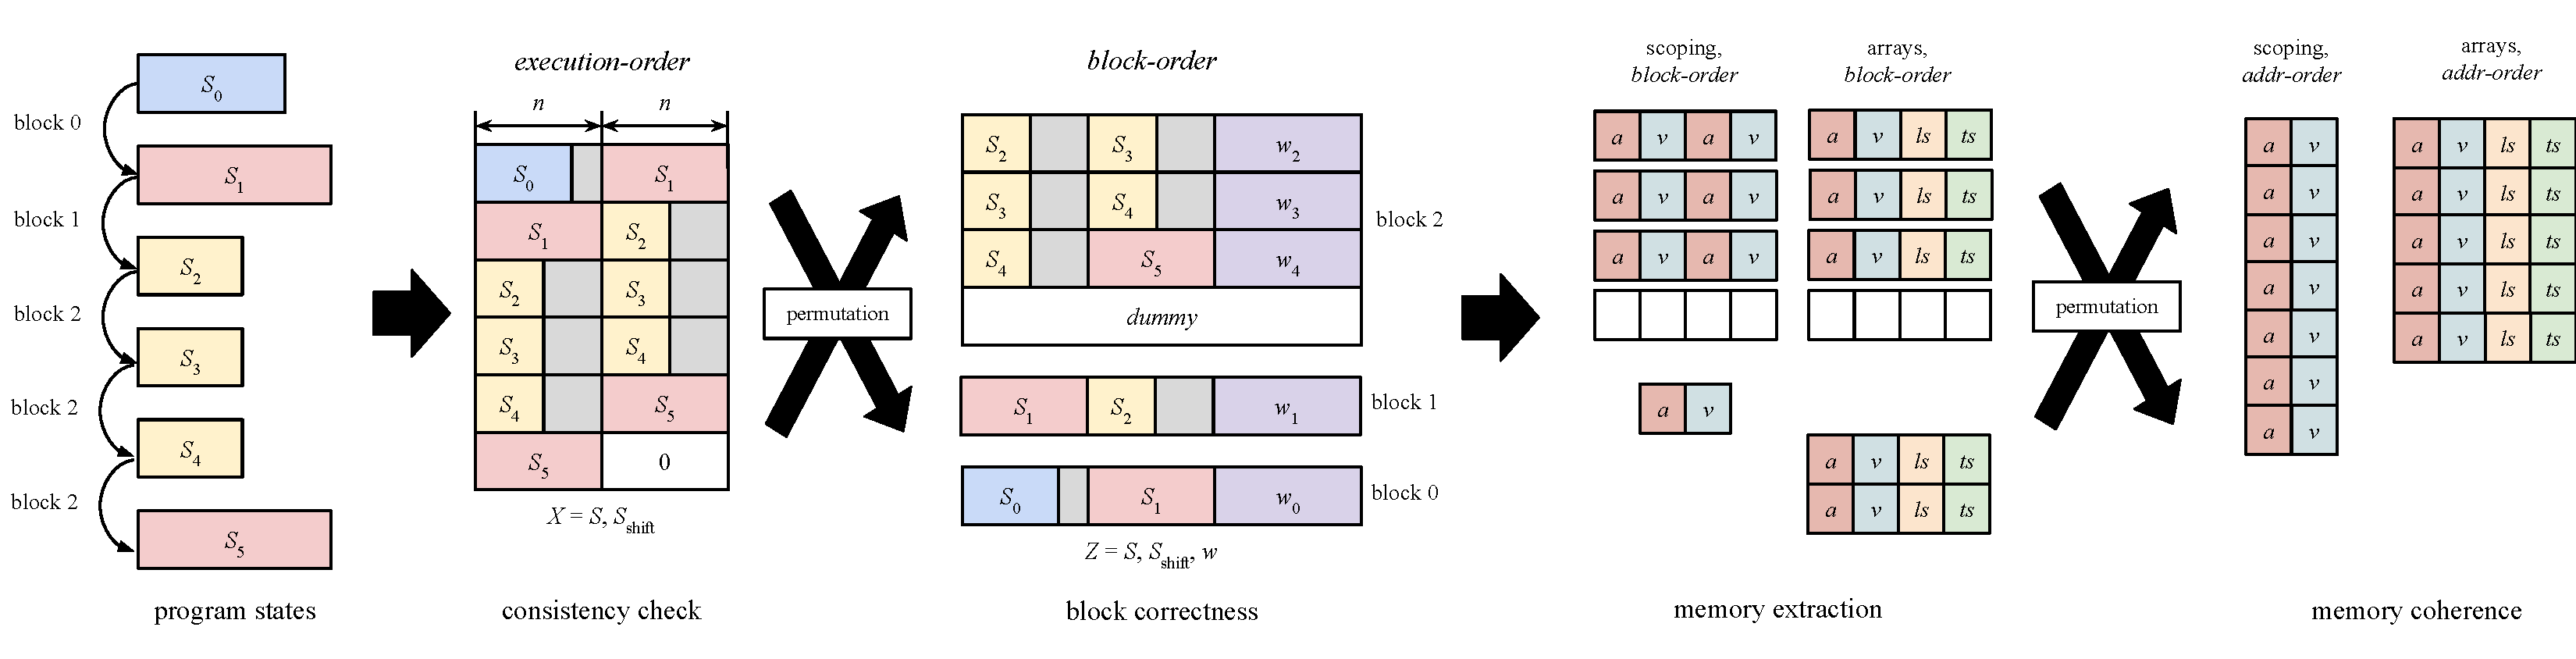
\includegraphics[width=\textwidth]{backend_overview.pdf}  
  \caption{Overview of the \CoBBl~backend.}
  \label{fig:backend-overview}
\end{figure*}

\subsection{Execution trace and witnesses}
For any execution of the \emph{preprocessed program}, \CoBBl~expresses the execution trace as a sequence of program states $[S_0\dots S_T]$, where $S_0$ is the program input and each subsequent state $S_{i+1}$ is produced by applying a block $I_i$ on the previous program state $S_i$. However, unlike vRAM, where each instruction sets a single output register, an execution of a block involves arbitrary side effects on all variables and an additional set of intermediate computations. As a result, to verify a block execution $I_i$, $\P$ computes $Z_i = (S_i, S_{i+1}, w_i)$ as witnesses for the proof, where $S_i$ is the prior program state and the input, $S_{i+1}$ is the next program state and the output, and $w_i$ contains all intermediate computations.

\subsection{Correct execution of blocks} \label{sec:block_correctness}
Verification of each individual block execution $I_i$, when singled out, is the exact same process as verifying a full program: a proof with constraints representing a block and witness represented as $Z_i = (S_i, S_{i+1}, w_i)$. Verification of multiple block executions in a data-paralleled proof, however, involves a few changes. The first is that, just like in vRAM, all executions of the same block need to be grouped together. This introduces a permutation described in section \ref{sec:perm}. Furthermore, number of executions of each block should be a power of 2 (or 0). These two properties allow the binary representation of the ordering to implicitly express the executed block. As an example, assume that the frontend emits 4 blocks: A, B, C, and D. For a particular computation, A is executed 8 times, B is executed 4 times, and C and D 2 times respectively. After sorting by block type, block correctness check verifies 16 executions in parallel, labeled as 0 to 15. To determine which block is applied to each program state, one refers to the binary of the label: if the first bit of the label is 0, then block A is in use; if the first two bits are 10, then B is in use, etc. Such implicit references avoid constraint description within each block execution.

Of course, the number of executions of most blocks are not a power of two. In this case $\P$ pads the proof with dummy executions where every witness is set to 0. This leads to a problem: constraints of every block need to be satisfiable by all-zero witnesses. Fortunately, this requirement is already satisfied by existing SNARK constraints, reasoned below:
\begin{itemize}
    \item If a constraint does not contain additions that involve constant values (i.e., it either performs arithmetic operations between witnesses, or multiplies a witness by a constant), then it can be satisfied by setting all witnesses to 0.
    \item To express additions with constant values, SNARK systems typically include a witness assigned to the constant 1 and perform addition using that witness. Since that witness is also set to 0 in a dummy execution, constraints with constant additions are also satisfiable by all-zero witnesses.
\end{itemize}

Finally, to ensure that $\P$ correctly sorts executions by block type, each block is assigned a label and each program state $S_i$ includes an additional register $\bn_i$ indicating the next block to be executed. Each block begins by checking that the value of $\bn_i$ matches with its label, and ends by setting $\bn_{i+1}$ to the label of the next block. If $\P$ incorrectly sorts or pads the executions, the check on $\bn_i$ fails, leading to a rejected proof.

\subsection{Consistency between program states} \label{sec:consistency}
The consistency check involves verifying that consecutive entries $Z_i = (S_i, s_{i+1}, w_i), Z_{i+1} = (S_{i+1}, s_{i+2}, w_{i+1})$ are consistent with each other, i.e. they share the same $S_{i+1}$. We note that $w_i$ plays no role in the consistency check, and does not need to be included. We pad each $S_i$ to width $n = \max_i|S_i|$. Let $X_i = (S_i, S_{i+1})$ so $|X_i| = 2n$, the goal of consistency check is to then show that
$$\forall k\in [0, n), X_i[n + k] = X_{i+1}[k]$$

Naively, the consistency proof seems easily parallelizable: each constraint of the consistency proof only uses variables from two consecutive entries $X_i$ and $X_{i+1}$. One can thus define the witnesses as $Y_i = (X_i, X_{i+1}) = (S_i, S_{i+1}, S_{i+1}, S_{i+2})$ and perform the following check in parallel across all $Y_i$:
$$\forall k\in [0, n), Y_i[n + k] = Y_i[2n + k]$$

However, such an approach only defers the problem from $X$ to $Y$. By expressing $Y_i = (X_i, X_{i+1})$, we now have to ask: how to prove that $Y_i$ and $Y_{i+1}$ share the same $X_{i+1}$?

Instead, \CoBBl~proves program state consistency through a \emph{proof of shift}. \CoBBl~represents each $X_i$ as a row in a $2n \times T$ matrix $X$. As shown in figure \ref{fig:backend-overview}, the matrix $X$ can be easily divided into two halfs: the left half is a matrix $S = S_0, \dots S_T$ and the right half is its shifted version $S_{\text{shift}} = S_1, \dots, S_T, 0$ differed by exactly one row ($n$ entries). \CoBBl~then generates the proof in the following manner:
\begin{enumerate}
    \item $\P$ provides $S$ and $S_{\text{shift}}$, and forms $X = S | S_{\text{shift}}$.
    \item $\P$ uses rows of $X$ as witnesses to produce a data-paralleled proof on program state consistency.
    \item $\P$ proves that $S_{\text{shift}}$ is $S$ shifted by $n$ entries.
\end{enumerate}

To prove that $S_{\text{shift}}$ is a shift of $S$, $\P$ interpolates both matrices as univariate polynomials $\tilde{S}, \tilde{S}_{\text{shift}}$ and evaluates them on a random point $r$. Let $\langle a, b \rangle$ denote vector dot product and
$$R = (1, r, r^2, r^3, \dots, r^n)$$
then
$$\tilde{S}(r) = \langle R, S_0 \rangle + r^n\cdot \langle R, S_1 \rangle + \dots + r^{(T-1)\cdot n} \langle R, S_T \rangle$$
$$\tilde{S}_{\text{shift}}(r) = \langle R, S_1 \rangle + r^n\cdot \langle R, S_2 \rangle + \dots + r^{(T-2)\cdot n} \langle R, S_T \rangle$$
So
$$\tilde{S}(r) = \langle R, S_0 \rangle + r^n \cdot \tilde{S}_{\text{shift}}(r)$$

Since $S_0$ is the program input already known by $\V$, $\V$ can manually compute $\langle R, S_0 \rangle$ and $r^n$. $\P$ provides $\tilde{S}(r)$ and $\tilde{S}_{\text{shift}}(r)$ through polynomial commitment, and $\V$ checks that $\tilde{S}(r) = \langle R, S_0 \rangle + r^n \cdot \tilde{S}_{\text{shift}}(r)$.

\bigskip
\noindent\textbf{Program input and output}. To conclude the consistency check, $\V$ needs to additionally check that the program input and output are correctly included in $S$. This is done by opening all relevant entries in $S_0$ and $S_T$ and verify their content.

\subsection{Permutation of program states} \label{sec:perm}
Since block execution check requires the program states to be sorted by block type, while consistency check requires the program states to be sorted by the order of execution, the next step is to verify that the two transcripts are indeed permutations of each other. Since the intermediate computations $w_i$ are only used in the block correctness proof, $w_i$ does not need to be part of the permutation. The permutation check is then reduced to the following problem: given two list of $(S_i, S_{i+1})$, how to prove that they are permutations of each other?

\CoBBl~reuses the idea of Reed-Solomon fingerprinting \cite{lipton90efficient}. Given two lists $a = (a_0, a_1, \dots, a_T), b = (b_0, b_1, \dots, b_T)$, to prove that they are permutations of each other, $\P$ constructs polynomials $A(i) = \prod_i(x - a_i)$ and $B(i) = \prod_i(x - b_i)$. $\V$ then evaluates them on a random point $\tau$. If $a$ and $b$ are permutations, then $A$ and $B$ are the same polynomial, so $A(\tau) = B(\tau)$. If $a$ and $b$ are not permutations, then $A$ and $B$ are different polynomials, and the likelihood of them agreeing on a random point is negligibly low.

To expand this idea onto $S$, where each entry of the lists are program states instead of a single number, $\CoBBl$ first performs \emph{the same random linear combination} on each program state to obtain $\text{RLC}(S_i) = \sum_k r^k s_{i, k}$. The remaining steps are now equivalent to that of a regular fingerprinting: construct two polynomials from $\text{RLC}_{\text{block}}$ and $\text{RLC}_{\text{exec}}$, and verify the equivalence of their evaluation on a random point $\tau$.

\subsection{Memory Coherence}
\CoBBl's memory coherence check closely resembles those of Buffet: for every load on an address, the value obtained should be the same as the last value loaded from or stored to that address. To verify this, \CoBBl~invokes a three-step process: extraction, permutation, and pairwise memory coherence check.

\paragraph{Extraction} The first step is to extract all memory accesses from the execution. As described in section \ref{sec:frontend_lowering}, memory accesses in \CoBBl~are separated into two categories: those on the scope stack and those on arrays. Operations on the scope stack are expressed using the pair $(\addr, \val)$, while operations on arrays are described by $(\addr, \val, \ls, \ts)$. Fortunately, since constraints for each block is fixed at compile time, for each block execution, \CoBBl~knows exactly where each memory variable is located. All that remains is for the frontend to append additional constraints to the end of each block, extracting out all scoping and array operations into a list of 2-tuples and a list of 4-tuples.

\paragraph{Permutation} The goal of the permutation is to allow $\P$ to sort all memory accesses by their addresses, on which the final coherence check will be performed. We note that this step is inherently identical to the process described in section \ref{sec:perm}. At the end of the permutation proof, $\P$ convinces $\V$ that a list of scoping accesses $L_{\text{scope}}$ and a list of array accesses $L_{\text{array}}$ contain all memory operations executed during the computation.

\paragraph{Pairwise coherence check} With lists of memory accesses purportedly sorted by their addresses, the final check is consisted of two steps. $\V$ first checks that the lists are sorted correctly: for $L_{\text{scope}}$, addresses should be increasing and differ by at most 1; for $L_{\text{array}}$, addresses should be increasing, and accesses on the same address is tie-breaked by the timestamp. The second check is on coherence: for $L_{\text{scope}}$, consecutive accesses on the same address should always result in the same value, and for consecutive accesses on the same address in $L_{\text{scope}}$, if the second access is a load, then the value of the second access should match that of the first. If both checks pass, then $\V$ is convinced of memory coherence.

%As a result, the proof includes the following witnesses from $\P$:
%\begin{itemize}
%    \item A list of program states $[S_0\dots S_T]$, sorted in the order of execution.
%    \item A list of consecutive program state pair $(S_i, S_{i+1})$, sorted by the type of block executed between the pair.
%    \item A list intermediate computations $z_i$ corresponding to the $(S_i, S_{i+1})$ pair.
%\end{itemize}
